% Chương 4 — Kết quả và phân tích. Số liệu kết quả để ở đây; phương pháp ở Chương 3.
% Nguồn số liệu mô hình (4.2–4.4): SERVER_CONTEXT/chapter3_evidence.md, chapter4_evidence.md, model_variant_fold_metrics.md,
% reports/P5-accuracy-coursework-summary.md, P5-accuracy-failure-analysis.md, P5-S2/S4/S6/S10-*.md.
% Mọi kết quả mô hình là development/exploratory; không có kết quả test niêm phong. Brier so sánh hiệu chỉnh
% tính ở mức item, không trọng số (src/hidden_dissatisfaction/modeling/training.py, _select_calibration).
\chapter{Kết quả và phân tích}\label{ch:results}

% =====================================================================
% Mục EDA. Nguồn số liệu: notebooks/olist_open_eda.ipynb (EDA mở), notebooks/01_eda_why_lateness_dominates.ipynb
% (5 lý do giao trễ chi phối), và script tính trên quần thể nghiên cứu dựng lại từ data/raw/olist theo đúng luật
% int_p4_cohort.sql + int_p4_review_canonical.sql (kết quả khớp tab:funnel: 85 420 đơn / 97 878 item).
% Hình sao chép từ notebooks/figures/ (nhãn tiếng Anh giữ nguyên).
\section{Kết quả phân tích khám phá dữ liệu}\label{sec:eda}

Trước khi huấn luyện mô hình, nhóm khảo sát dữ liệu để trả lời hai câu hỏi. Câu thứ nhất là dữ liệu có đủ tin cậy để dựng quần thể và đặc trưng như mô tả ở Chương~\ref{ch:method} hay không; câu thứ hai là trong nhóm đơn giao đúng hạn còn lại những tín hiệu nào gắn với đánh giá thấp. Số liệu trong mục này thuộc ba mẫu khác nhau, và mỗi con số đều được ghi rõ mẫu của nó như sau.
\begin{itemize}
  \item \emph{Toàn bộ dữ liệu} Olist: 99\,441 đơn.
  \item \emph{Mẫu đã giao có đánh giá}: 95\,824 đơn đã giao, có ngày giao và có đánh giá, dùng khi so sánh đơn trễ với đơn đúng hạn. Ở mẫu này, một đơn được xem là trễ khi \emph{ngày} giao muộn hơn ngày dự kiến.
  \item \emph{Quần thể nghiên cứu} theo Bảng~\ref{tab:funnel}: 85\,420 đơn với 97\,878 item, dựng lại từ tệp CSV gốc bằng đúng luật lọc và luật chọn đánh giá của kho dữ liệu. Quần thể này so sánh ngày giao với ngày dự kiến theo mốc thời gian đầy đủ, nên số đơn ``đúng hạn'' của nó chênh vài nghìn đơn so với cách đếm theo ngày. Snapshot dùng để huấn luyện lệch so với bản dựng lại 5 đơn và 6 item.
\end{itemize}
Mọi kết quả trong mục là mô tả và tương quan, không mang ý nghĩa nhân quả.

\subsection{Độ phủ thời gian và chất lượng dữ liệu}\label{subsec:eda-coverage}

Dữ liệu Olist trải từ tháng 9/2016 đến tháng 10/2018 nhưng chỉ 20 tháng có mật độ đủ để phân tích (Hình~\ref{fig:eda-coverage}, các tháng tô xám là giai đoạn quá thưa). Từ tháng 1/2017 đến tháng 8/2018 có 99\,092 trong tổng số 99\,441 đơn. Năm 2016 gần như trống (tháng 11/2016 không có đơn nào), còn 20 đơn của tháng 9--10/2018 chưa từng được giao. Lượng đơn tăng nhanh trong năm 2017 rồi đi ngang ở mức 6\,200--7\,300 đơn mỗi tháng suốt năm 2018; tám tháng đầu năm 2018 có 53\,991 đơn, gấp khoảng 2,35 lần cùng kỳ năm 2017 (22\,968 đơn). Ngày Black Friday 24/11/2017 ghi nhận 1\,176 đơn, trong khi trung vị một ngày năm 2018 chỉ là 227 đơn. Vì năm 2016 quá thưa, phân vùng huấn luyện ở Bảng~\ref{tab:split} tuy bắt đầu từ tháng 10/2016 nhưng phần lớn dữ liệu của nó thuộc năm 2017.

\begin{figure}[htbp]\centering
  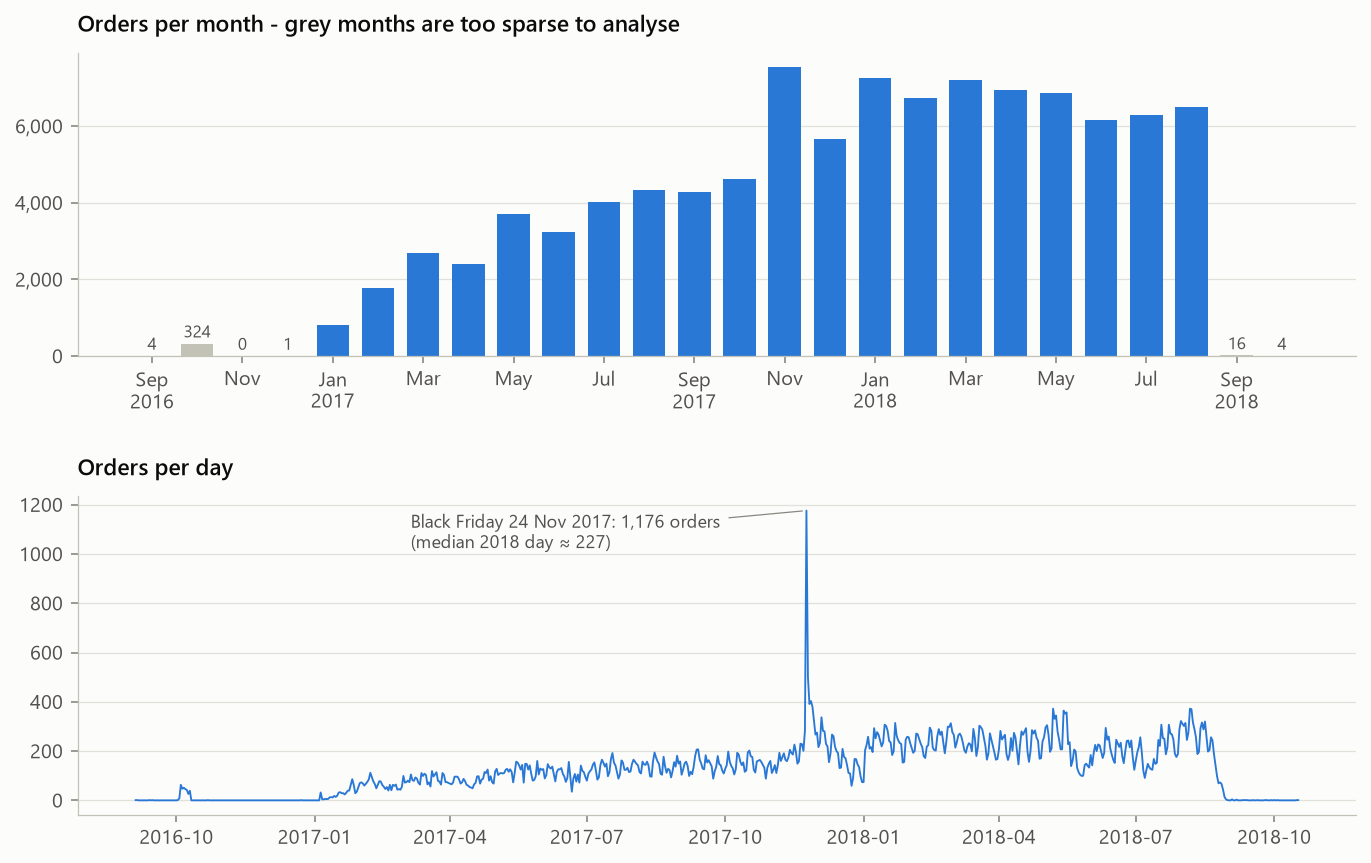
\includegraphics[width=\linewidth]{eda/01_coverage}
  \caption{Số đơn Olist theo tháng và theo ngày}
  \label{fig:eda-coverage}
\end{figure}

Hành vi vận hành cũng không đứng yên theo thời gian (Hình~\ref{fig:eda-operations}, tính theo tháng mua trên các đơn đã giao). Tỉ lệ giao trễ chỉ 3--5\% trong các tháng bình thường nhưng lên 12,4\% với đơn mua tháng 11/2017, 14,1\% với tháng 2/2018 và 19,0\% với tháng 3/2018 (vùng tô xám trong hình); điểm đánh giá trung bình giảm tương ứng xuống 3,91, 3,83 và 3,75, so với khoảng 4,2 ở các tháng khác. Thời gian giao dự kiến (trung vị) giảm từ 39 ngày vào tháng 1/2017 xuống khoảng 23 ngày từ giữa năm 2017 và còn 13,4 ngày vào tháng 8/2018. Cuộc đình công của tài xế xe tải cuối tháng 5/2018 kéo số đơn giao mỗi tuần từ khoảng 2\,000 xuống 634, và số người bán hoạt động mỗi tháng tăng từ 227 lên 1\,278. Những thay đổi chế độ vận hành này là bằng chứng trực tiếp cho lựa chọn chia dữ liệu theo thời gian thay vì chia ngẫu nhiên ở Chương~\ref{ch:method}, bởi một phép chia ngẫu nhiên sẽ trộn các giai đoạn có quy tắc hứa giao và tỉ lệ trễ rất khác nhau.

\begin{figure}[htbp]\centering
  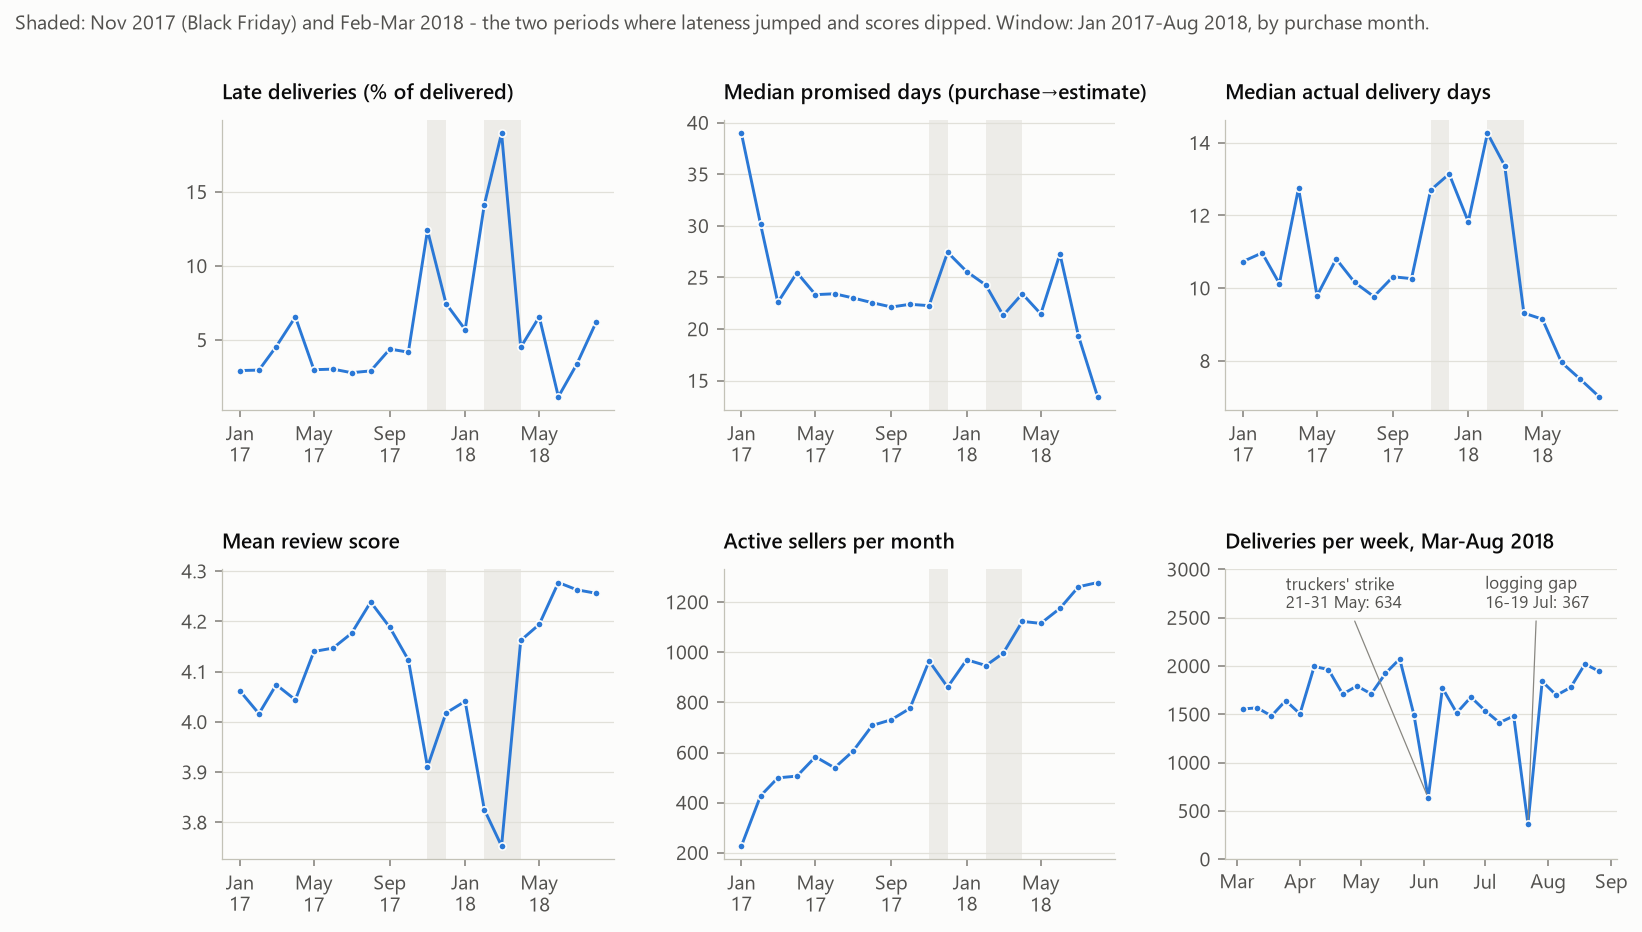
\includegraphics[width=\linewidth]{eda/03_operations_over_time}
  \caption{Diễn biến vận hành theo tháng mua}
  \label{fig:eda-operations}
\end{figure}

Kiểm tra chất lượng dữ liệu cho thấy bộ Olist nhìn chung sạch, nhưng có một số bẫy ảnh hưởng trực tiếp đến cách dựng quần thể. Nếu nối thẳng bảng đơn với bảng sản phẩm, thanh toán và đánh giá mà không gộp trước, kết quả có 117\,329 dòng cho 97\,916 đơn và doanh thu sản phẩm bị đếm thành 14,14 triệu real thay vì 13,59 triệu, đúng hiện tượng nhân bản dòng đã nêu ở Chương~\ref{ch:method}. Có 547 đơn mang 2--3 đánh giá, trong đó 202 đơn có các điểm số không thống nhất, nên cần một luật chọn đánh giá tất định như mô tả ở Chương~\ref{ch:method}; ngoài ra 789 mã đánh giá được dùng chung cho nhiều đơn, nên không thể khử trùng chỉ theo mã đánh giá.

Các mốc thời gian cũng có điểm bất thường. Có 1\,359 đơn có mốc bàn giao vận chuyển sớm hơn mốc duyệt thanh toán và 23 đơn có mốc giao cho khách sớm hơn mốc bàn giao; các khoảng thời gian âm này cần được đánh dấu thay vì tin tưởng. Hai khoảng 16--19/7/2018 và ngày 20/6/2017 gần như không có đơn được ghi nhận giao dù việc bàn giao vận chuyển vẫn diễn ra bình thường, nhiều khả năng là khoảng trống ghi log. Trong 96\,470 đơn đã giao có ngày giao, ngoài bình luận tùy chọn thì chỉ danh mục sản phẩm (1,41\%), đánh giá (0,67\%) và khoảng cách giữa người bán và khách hàng (0,49\%) có tỉ lệ thiếu đáng kể. Ở các bảng phụ, 610 sản phẩm không có danh mục, 26,2\% số dòng tọa độ là bản trùng hoàn toàn và 42 điểm tọa độ nằm ngoài lãnh thổ Brazil.

\subsection{Phân bố điểm đánh giá và mức mất cân bằng lớp}\label{subsec:eda-labels}

Điểm đánh giá có dạng chữ J quen thuộc (Hình~\ref{fig:eda-reviews}). Trên toàn bộ 99\,224 dòng đánh giá, 57,8\% là 5 sao, 19,3\% là 4 sao, 8,2\% là 3 sao, 3,2\% là 2 sao và 11,5\% là 1 sao. Khách không hài lòng viết bình luận nhiều hơn hẳn, với 77\% đánh giá 1 sao có bình luận so với 31\% ở mức 4 sao. Bình luận dồn ứ ở đúng 200 ký tự (659 bình luận), dấu hiệu văn bản đã bị cắt ngắn.

\begin{figure}[htbp]\centering
  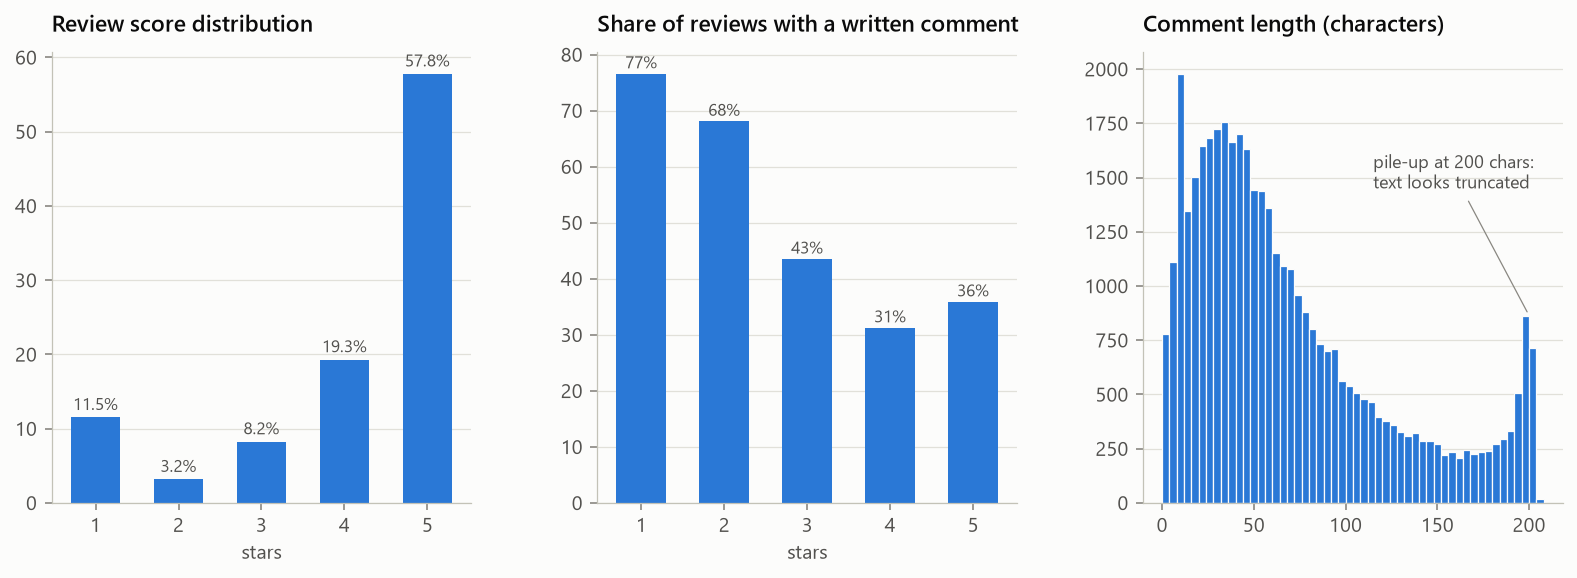
\includegraphics[width=\linewidth]{eda/13_reviews_overview}
  \caption{Phân bố điểm và bình luận đánh giá}
  \label{fig:eda-reviews}
\end{figure}

Trong quần thể nghiên cứu, phân bố dịch về phía hài lòng, với 62,45\% đơn nhận 5 sao, 20,35\% nhận 4 sao, 8,00\% nhận 3 sao, 2,63\% nhận 2 sao và 6,58\% nhận 1 sao. Tỉ lệ dương ở mức đơn vì vậy là 9,21\% (7\,865/85\,420), thấp hơn đáng kể so với 14,69\% khi tính trên mọi đơn có đánh giá. Ở mức item, tỉ lệ dương lên tới 11,41\% vì đơn nhiều sản phẩm có tỉ lệ bị đánh giá thấp cao hơn (mục~\ref{subsec:eda-ontime}) và đóng góp nhiều dòng hơn.

Khác biệt giữa hai mức này cần được ghi nhớ khi đọc Bảng~\ref{tab:split}. Tỉ lệ dương 10,13--13,80\% trong bảng đó được tính ở mức item, còn nếu dựng lại theo cùng mốc thời gian ở mức đơn thì tỉ lệ dương của năm phân vùng phát triển là 8,86--10,53\%. Theo tháng giao, tỉ lệ dương mức đơn của quần thể nghiên cứu dao động trong khoảng 7,8--10,9\%. Với khoảng một đơn dương trên mười một đơn, accuracy không phải thước đo phù hợp, như đã lập luận ở mục~\ref{sec:th-metrics}; tỉ lệ dương mức đơn này cũng là mốc ngẫu nhiên khi đọc PR-AUC ở mục~\ref{sec:results-analysis}.

\subsection{Vì sao giao trễ chi phối các mô hình dự báo hiện có}\label{subsec:eda-lateness}

Trên các đơn đã giao có đánh giá, giao trễ là tín hiệu mạnh nhất của đánh giá thấp. Theo định nghĩa trễ theo ngày, 6,7\% đơn bị giao trễ, và nhóm này có 62,4\% đơn bị đánh giá 1--2 sao, gấp 6,7 lần tỉ lệ 9,3\% của đơn đúng hạn. Hình~\ref{fig:eda-factors} đặt tám yếu tố trên cùng một thang đo, với đường xám là tỉ lệ chung 14,7\% trên mọi đơn có đánh giá; các ô về thời gian giao và khoảng cách chỉ tính trên đơn đã giao. Tỉ lệ đánh giá thấp chỉ 9\% với đơn giao sớm từ 7 ngày trở lên và 11\% với đơn giao sớm 0--6 ngày, nhưng lên 32\% khi trễ 1--3 ngày, 68\% khi trễ 4--7 ngày và 79\% khi trễ hơn 7 ngày. Quan hệ này có dạng bậc thang. Giao sớm hơn hứa hẹn hầu như không cải thiện thêm, nhưng chỉ cần vượt qua ngày hứa là tỉ lệ tăng vọt. Theo bảng chi tiết của notebook, tỉ lệ đánh giá thấp là 12,4\% với đơn giao đúng ngày dự kiến, 19,6\% khi trễ một ngày và 50,4\% khi trễ ba ngày. Dạng bất đối xứng này khớp với kết quả của \textcite{ravula2023} và với bằng chứng về tác động của chất lượng giao hàng lên điểm đánh giá~\parencite{deshpande2023}.

\begin{figure}[htbp]\centering
  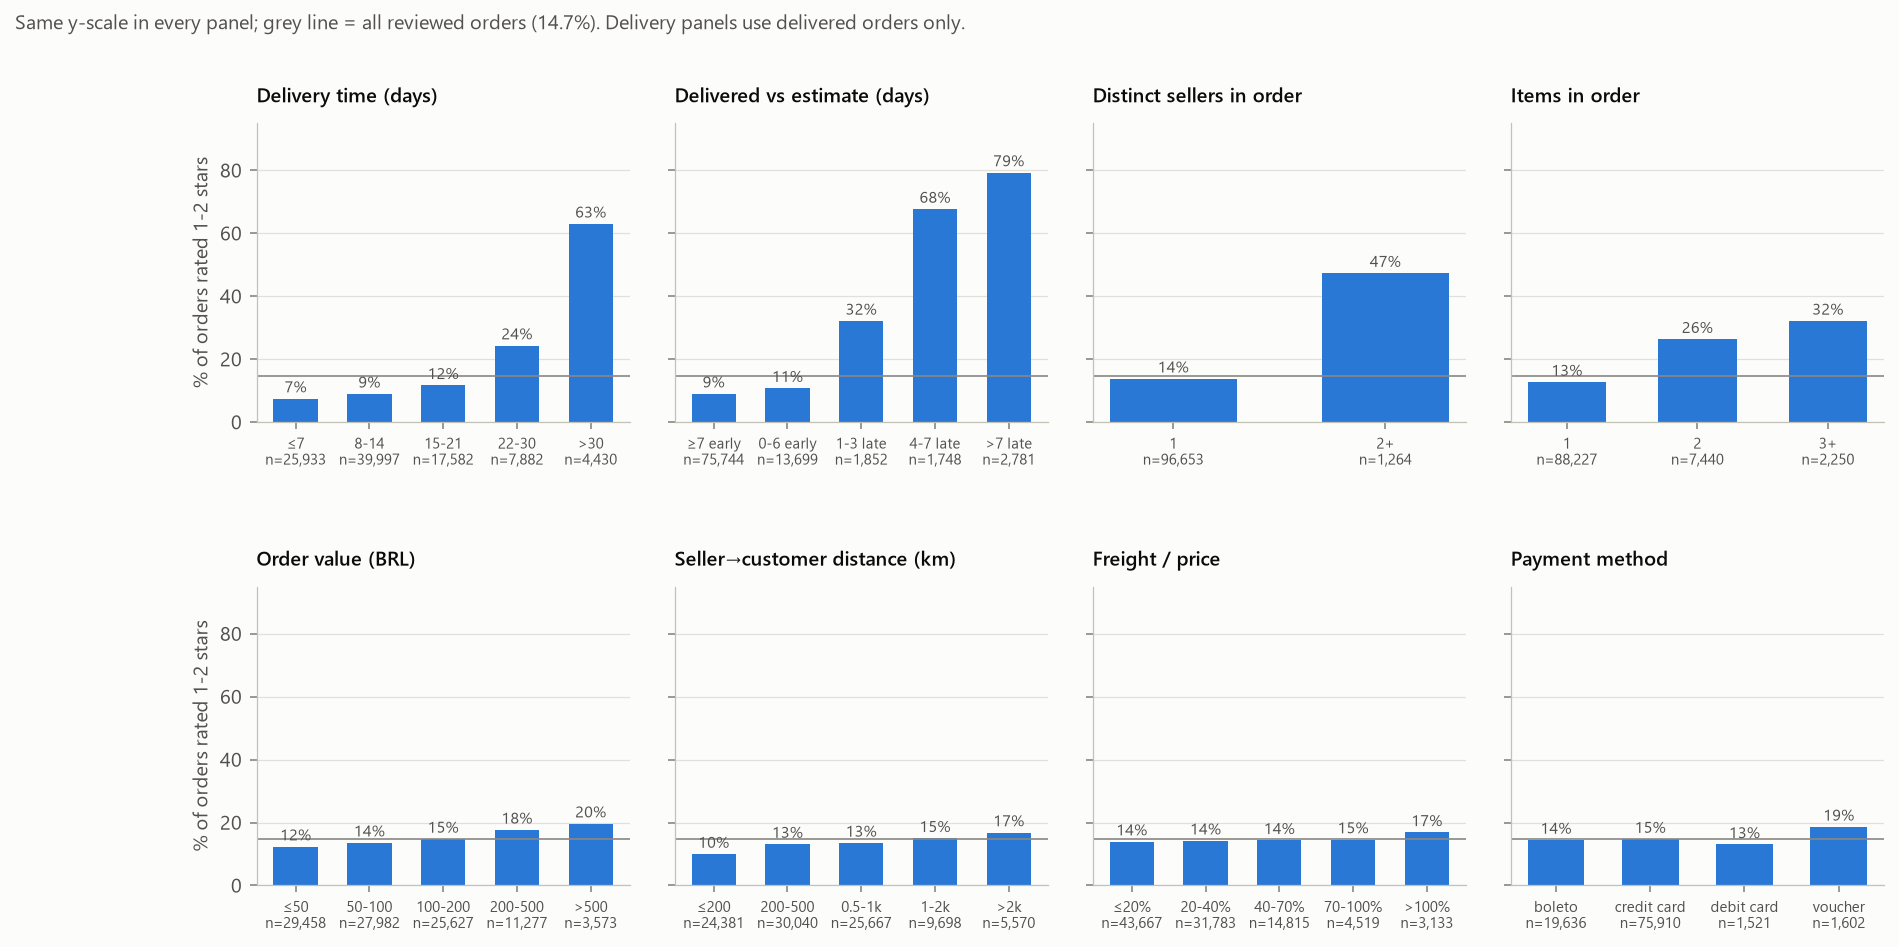
\includegraphics[width=\linewidth]{eda/14_score_factors}
  \caption{Tỉ lệ đánh giá 1--2 sao theo tám yếu tố}
  \label{fig:eda-factors}
\end{figure}

Phân tích trong notebook chỉ ra năm lý do khiến các mô hình hài lòng trên Olist hầu như đều ``phát hiện'' giao trễ là yếu tố quyết định (Bảng~\ref{tab:eda-reasons}). Lý do thứ hai đáng chú ý nhất vì nó nằm ở cơ chế sinh nhãn. Olist gửi khảo sát khi khách nhận hàng \emph{hoặc} khi đến ngày giao dự kiến~\parencite{olist2018}, nên với đơn trễ, khách thường được hỏi về một món hàng chưa nhận được. Trong mẫu đơn trễ, 70,1\% đánh giá được trả lời trước khi hàng đến và 80,8\% số đánh giá này là 1--2 sao; ngược lại, ở đơn đúng hạn chỉ 0,3\% khảo sát được gửi trước ngày giao. Với phần lớn đơn trễ, ``đánh giá'' thực chất là lời phàn nàn hàng chưa tới, và dự báo nó từ mốc thời gian gần như là dự báo lịch gửi khảo sát. Quần thể nghiên cứu loại bỏ vấn đề này từ gốc, vì chỉ giữ đơn giao đúng hạn và có đánh giá tạo sau thời điểm giao.

\begin{table}[htbp]\centering\small
\caption{Năm lý do giao trễ chi phối các mô hình dự báo hài lòng trên Olist (mẫu: 95\,824 đơn đã giao có đánh giá; trễ tính theo ngày)}\label{tab:eda-reasons}
\begin{tabular}{p{4.3cm}p{9.2cm}}
\toprule
Lý do & Bằng chứng \\
\midrule
Giao trễ là tín hiệu mạnh và có dạng bậc thang & 62,4\% đơn trễ bị đánh giá thấp so với 9,3\% đơn đúng hạn; trễ ba ngày đã có 50,4\% đơn bị đánh giá thấp (Hình~\ref{fig:eda-factors}) \\
Nhãn của đơn trễ phần lớn do lịch gửi khảo sát tạo ra & 70,1\% đánh giá của đơn trễ được viết trước khi hàng đến, 80,8\% trong số đó là 1--2 sao \\
Giao trễ quyết định các biến động theo thời gian & Tỉ lệ đánh giá thấp toàn bộ dao động 9,4--21,2\% theo tháng và tăng cùng tỉ lệ trễ (14,0\% tháng 2/2018, 18,7\% tháng 3/2018); tỉ lệ ở đơn đúng hạn chỉ dao động 7,4--10,7\% \\
Đặc trưng thời gian đứng đầu khi gộp mọi đơn & ROC-AUC đơn biến của bốn đặc trưng thời gian đứng đầu là 0,65--0,69 trên mọi đơn, nhưng các đặc trưng này chỉ đạt 0,51--0,57 trên đơn đúng hạn; ở nhóm này số item trong đơn (0,59), tỉ lệ đánh giá thấp trước đó của người bán (0,59) và phí vận chuyển (0,58) dẫn đầu \\
Accuracy che giấu vấn đề & Một mô hình boosting chẩn đoán (chia ngẫu nhiên 70/30, ngưỡng 0,5, như các nghiên cứu trước) đạt accuracy 89,8\%, chỉ hơn mức luôn dự đoán ``không tiêu cực'' (87,2\%) 2,6 điểm; 58,7\% danh sách 10\% rủi ro cao nhất là đơn trễ dù đơn trễ chỉ chiếm 6,7\%, và danh sách này bắt được 96,5\% đơn trễ bị đánh giá thấp nhưng chỉ 16,7\% đơn đúng hạn bị đánh giá thấp \\
\bottomrule
\end{tabular}
\end{table}

Hệ quả là các mô hình huấn luyện trên mọi đơn học chủ yếu cách nhận diện đơn trễ, trong khi phần lớn đánh giá thấp lại nằm ở nhóm còn lại. Trong 12\,272 đơn bị đánh giá 1--2 sao thuộc mẫu đã giao có đánh giá, 8\,289 đơn (67,5\%) đến từ đơn giao đúng hạn theo định nghĩa theo ngày; dùng định nghĩa theo mốc thời gian của quần thể nghiên cứu, con số là 8\,130 đơn (66,25\%). Đơn đúng hạn cũng là trạng thái phổ biến chứ không phải ngoại lệ (Hình~\ref{fig:eda-promise}). Trung vị thời gian giao thực tế là 10,2 ngày so với 23,2 ngày hứa giao, và 93,2\% đơn đến đúng hoặc sớm hạn với trung vị sớm 12 ngày. Theo tháng, tỉ lệ đánh giá thấp của đơn đúng hạn chỉ dao động trong khoảng 7,4--10,7\% (Bảng~\ref{tab:eda-reasons}), nên nhóm khách này không bao giờ hiện lên thành một đỉnh trên biểu đồ vận hành. Đó chính là lý do sự bất mãn của họ được gọi là ``ẩn''.

\begin{figure}[htbp]\centering
  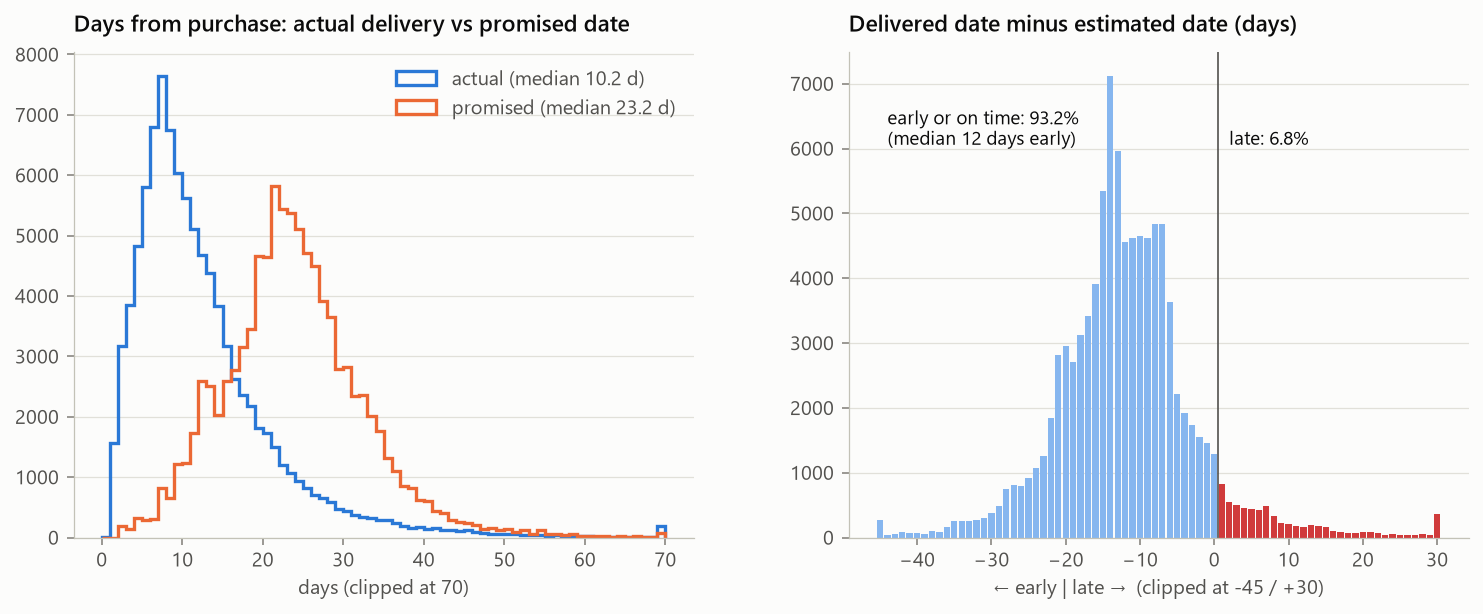
\includegraphics[width=\linewidth]{eda/09_promise_vs_reality}
  \caption{Thời gian giao thực tế so với thời gian hứa giao}
  \label{fig:eda-promise}
\end{figure}

\subsection{Tín hiệu trong nhóm đơn giao đúng hạn}\label{subsec:eda-ontime}

Khi đã loại giao trễ, các tín hiệu còn lại yếu hơn nhưng không biến mất. Bảng~\ref{tab:eda-segments} tóm tắt tỉ lệ đánh giá thấp mức đơn trong quần thể nghiên cứu theo các yếu tố đều biết được tại thời điểm giao. Cấu trúc đơn tạo khác biệt lớn nhất. Đơn có hai người bán bị đánh giá thấp 45,7\%, gấp hơn năm lần đơn một người bán (8,7\%), và tỉ lệ tăng đều từ 7,5\% ở đơn một item lên 31,9\% ở đơn từ bốn item. Nhóm đơn nhiều người bán rất nhỏ (1\,214 đơn), nhưng tỉ lệ 45,7--63,2\% của nó đã ngang với mức 62,4\% của đơn \emph{trễ} ở mục~\ref{subsec:eda-lateness}. Ở toàn bộ dữ liệu, đơn nhiều người bán còn có tỉ lệ trễ ghi nhận chỉ 1,0\% so với 6,9\% của đơn một người bán và điểm trung bình 2,86 so với 4,12, cho thấy mốc giao duy nhất của đơn nhiều khả năng chỉ phản ánh kiện hàng đến trước. Quan sát này khớp với bằng chứng rằng giao hàng tách kiện làm giảm sự hài lòng~\parencite{brylla2022}.

\begin{table}[htbp]\centering\small
\caption{Tỉ lệ đơn bị đánh giá 1--2 sao trong quần thể nghiên cứu theo một số yếu tố biết được tại thời điểm giao (85\,420 đơn dựng lại; tỉ lệ chung 9,21\%; mỗi yếu tố chỉ trình bày một số nhóm tiêu biểu)}\label{tab:eda-segments}
\begin{tabular}{llrr}
\toprule
Yếu tố & Nhóm & Số đơn & Tỉ lệ đánh giá thấp \\
\midrule
Số người bán trong đơn & 1 & 84\,206 & 8,7\% \\
 & 2 & 1\,157 & 45,7\% \\
 & 3 trở lên & 57 & 63,2\% \\
\addlinespace
Số item trong đơn & 1 & 76\,678 & 7,5\% \\
 & 2 & 6\,695 & 23,2\% \\
 & 3 & 1\,191 & 27,0\% \\
 & 4 trở lên & 856 & 31,9\% \\
\addlinespace
Số ngày từ mua đến giao & $\le$3 & 4\,622 & 6,6\% \\
 & 7--14 & 38\,328 & 8,7\% \\
 & 21--30 & 5\,164 & 14,6\% \\
 & $>$30 & 786 & 22,4\% \\
\addlinespace
Số ngày giao sớm so với dự kiến & 0--3 & 4\,505 & 11,3\% \\
 & 14--21 & 23\,515 & 8,3\% \\
 & $>$30 & 2\,256 & 11,0\% \\
\addlinespace
Bàn giao vận chuyển sau hạn & Không & 79\,118 & 8,9\% \\
 & Có & 6\,302 & 13,6\% \\
\addlinespace
Giá trị sản phẩm (real) & $\le$50 & 25\,911 & 7,8\% \\
 & $>$500 & 3\,020 & 12,9\% \\
\addlinespace
Phí vận chuyển / giá & $\le$20\% & 38\,050 & 8,8\% \\
 & $>$100\% & 2\,663 & 10,6\% \\
\addlinespace
Thanh toán đầu tiên & Thẻ tín dụng & 65\,863 & 9,2\% \\
 & Boleto & 16\,904 & 9,2\% \\
 & Voucher & 1\,342 & 10,5\% \\
\bottomrule
\end{tabular}
\end{table}

Đúng hạn không đồng nghĩa với nhanh. Đơn giao trong vòng ba ngày bị đánh giá thấp 6,6\%, còn đơn mất hơn 30 ngày dù vẫn kịp hạn có tỉ lệ 22,4\%. Khách đánh giá cả độ dài thời gian chờ chứ không chỉ việc lời hứa có được giữ hay không. Khoảng dư so với ngày dự kiến lại có dạng chữ U. Đơn kịp hạn sát nút (0--3 ngày) có tỉ lệ 11,3\%, đơn sớm 14--21 ngày có tỉ lệ thấp nhất 8,3\%, và đơn sớm hơn 30 ngày tăng trở lại 11,0\%, nhiều khả năng vì những đơn này đi kèm thời hạn hứa giao rất dài. Người bán bàn giao vận chuyển sau hạn gửi hàng nhưng hàng vẫn đến kịp có tỉ lệ 13,6\%, so với 8,9\% ở trường hợp còn lại. Lịch sử của người bán cũng mang tín hiệu. Trên mẫu đơn đúng hạn theo ngày của notebook (89\,443 đơn), người bán có hơn 30\% đánh giá thấp trong quá khứ tạo ra 18,4\% đánh giá thấp, so với 6,5\% ở người bán có tỉ lệ quá khứ từ 5\% trở xuống; tỉ lệ quá khứ này chỉ tính trên các đánh giá đã có trước thời điểm mua.

Danh mục sản phẩm tạo khác biệt vừa phải. Tính ở mức item trong quần thể nghiên cứu với các danh mục có từ 800 item, nội thất văn phòng có tỉ lệ dương cao nhất (22,4\% trên 1\,460 item), tiếp theo là đồ trang trí nội thất (14,9\%), chăn ga gối (14,8\%) và phụ kiện máy tính (14,0\%); thấp nhất là phụ kiện hành lý (6,5\%) và văn phòng phẩm (7,6\%). Các item thiếu danh mục có tỉ lệ 15,1\% (1\,344 item), vì vậy giữ ``thiếu danh mục'' thành một nhóm riêng có lợi hơn là điền giá trị. Các yếu tố tiền tệ dịch chuyển ít hơn. Tỉ lệ tăng từ 7,8\% ở đơn dưới 50 real lên 12,9\% ở đơn trên 500 real, còn tỉ trọng phí vận chuyển (8,8--10,6\%) và phương thức thanh toán (8,5--10,5\%) gần như phẳng. Theo bang của khách (các bang có từ 1\,000 đơn), tỉ lệ dao động từ 8,6\% ở São Paulo đến 10,9\% ở Rio de Janeiro và 11,1\% ở Bahia.

Ma trận tương quan Spearman trên 96\,470 đơn đã giao cho thấy vì sao các tín hiệu này khó nắm bắt bằng quan hệ tuyến tính. Không biến số mức đơn nào có hệ số tương quan Spearman với điểm đánh giá vượt quá 0,25 về độ lớn; mạnh nhất là số ngày giao ($-0{,}23$), thời gian vận chuyển ($-0{,}19$), chênh lệch so với ngày dự kiến ($-0{,}18$) và số item ($-0{,}11$). Các quan hệ ở Bảng~\ref{tab:eda-segments} có dạng ngưỡng hoặc chữ U, điều mà tương quan đơn điệu đánh giá thấp. Nhiều cặp biến giải thích lại đi cùng nhau, như số ngày giao và thời gian vận chuyển ($0{,}89$), giá trị đơn và tỉ trọng phí vận chuyển ($-0{,}78$), khoảng cách và số ngày hứa giao ($0{,}62$). Mô hình tuyến tính vì thế dễ gặp đa cộng tuyến, còn mô hình cây có thể tách các ngưỡng mà không cần chỉ định trước dạng quan hệ.

\subsection{Nội dung đánh giá của khách không hài lòng}\label{subsec:eda-text}

Văn bản đánh giá chỉ xuất hiện \emph{sau} khi khách đánh giá, nên nó không được dùng làm đặc trưng (Hình~\ref{fig:leakage-timeline}); nhóm chỉ dùng nó để hiểu nhãn. Theo luật từ khóa trên bình luận tiếng Bồ Đào Nha đã bỏ dấu (Hình~\ref{fig:eda-themes}), bình luận 1 sao chủ yếu nói hàng chưa tới (31\%), sau đó là hoàn tiền, trả hàng hoặc hủy đơn (10\%), thiếu một phần đơn (9\%), giao chậm (7\%), lỗi hoặc hư hỏng (6\%) và giao sai sản phẩm (6\%). Bình luận 4--5 sao thì xoay quanh giao nhanh và lời khen. Bình luận của đơn nhiều người bán khác hẳn, với 31,3\% nói thiếu một phần đơn và 29,8\% nói chưa nhận được hàng, so với 3,0\% và 8,3\% ở đơn một người bán.

\begin{figure}[htbp]\centering
  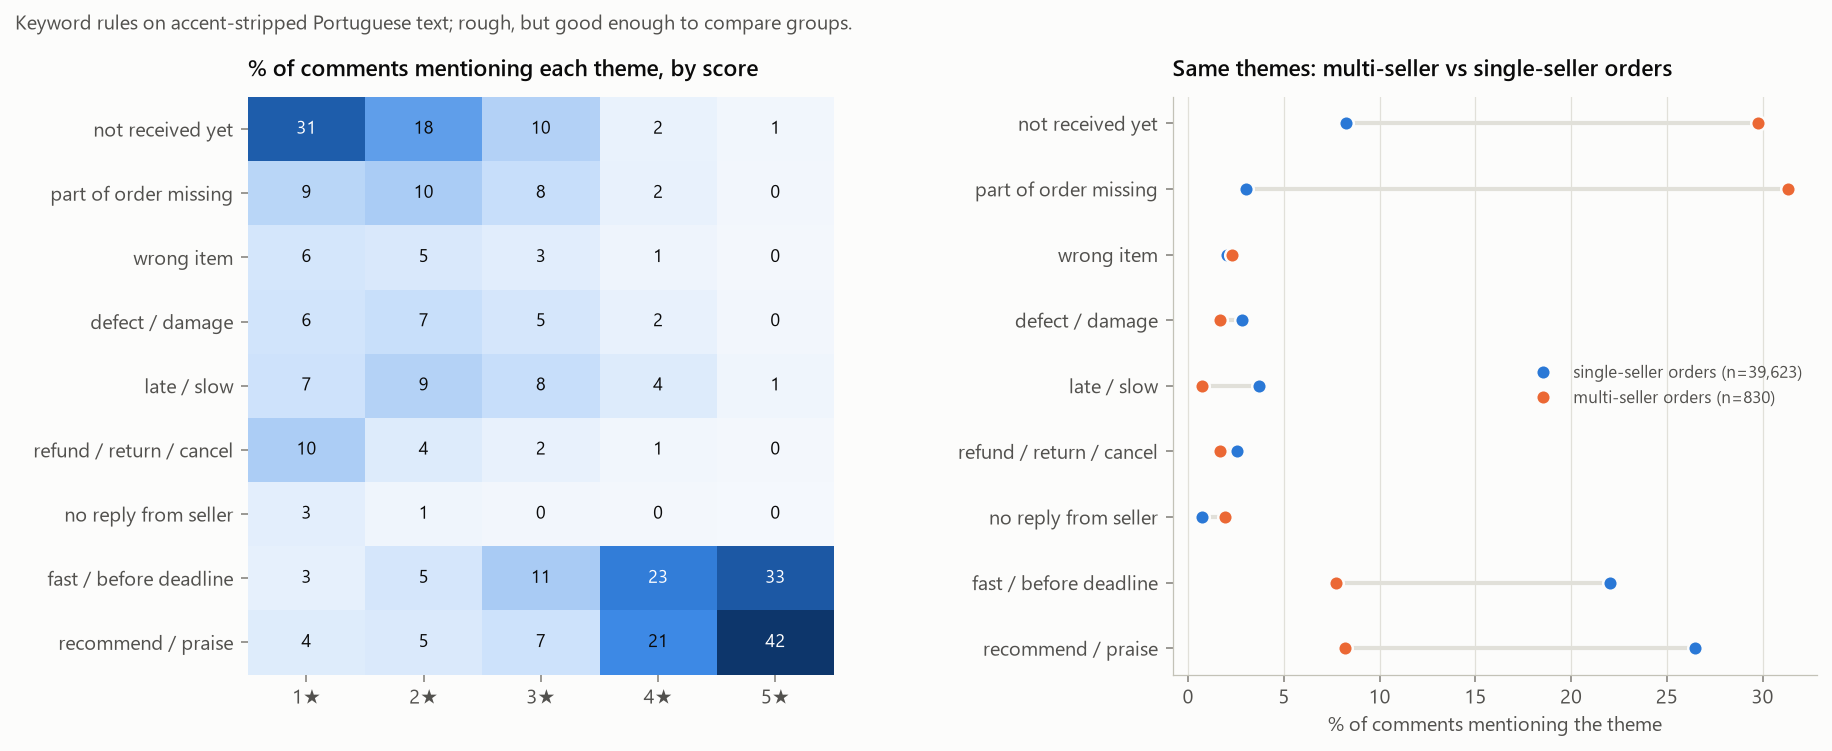
\includegraphics[width=\linewidth]{eda/15_text_themes}
  \caption{Chủ đề trong bình luận đánh giá}
  \label{fig:eda-themes}
\end{figure}

So sánh bình luận tiêu cực của đơn trễ và đơn đúng hạn làm rõ khác biệt về bản chất. Trong 2\,747 bình luận 1--2 sao của đơn trễ, 52,4\% nói chưa nhận được hàng và chỉ 2,0\% nói hàng sai, khác mô tả, lỗi hoặc vỡ. Trong 6\,487 bình luận 1--2 sao của đơn đúng hạn, hai tỉ lệ này lần lượt là 13,9\% và 17,9\%, và 20,3\% nói chỉ nhận được một phần đơn; riêng đơn đúng hạn có từ hai người bán, tỉ lệ nói thiếu một phần lên 51,9\%. Có 78,3\% đánh giá thấp của đơn đúng hạn kèm bình luận. Nói cách khác, khách phàn nàn về đơn trễ vì hàng \emph{chưa đến}, còn khách phàn nàn về đơn đúng hạn vì \emph{thứ đã đến} bị thiếu, sai, hỏng hoặc kém chất lượng. Không vấn đề nào trong số này lộ ra qua chênh lệch giữa ngày giao và ngày dự kiến.

\subsection{Hàm ý cho thiết kế đặc trưng}\label{subsec:eda-implications}

Kết quả khám phá dữ liệu định hướng trực tiếp các nhóm đặc trưng ở Bảng~\ref{tab:features}. Tín hiệu mạnh nhất trong nhóm đúng hạn đến từ cấu trúc đơn, nên số người bán, số danh mục, số sản phẩm, các cờ nhiều item, nhiều người bán, nhiều danh mục và chỉ số tập trung Herfindahl--Hirschman được tách thành ba nhóm riêng. Do Olist chỉ có một mốc giao cho mỗi đơn, các đặc trưng này đóng vai trò đại diện gián tiếp cho việc giao thiếu hoặc tách kiện mà bình luận phản ánh. Thời gian giao thực tế, thời gian vận chuyển và khoảng dư so với ngày dự kiến được giữ trong nhóm cơ sở vì đơn chờ lâu vẫn có rủi ro cao dù kịp hạn; quan hệ chữ U của khoảng dư là thêm một lý do để ưu tiên mô hình cây.

Lịch sử đánh giá của người bán và danh mục, cùng nhóm tốc độ và độ biến động của người bán, khai thác tín hiệu từ người bán bàn giao trễ và người bán có tiền sử bị đánh giá thấp; cả hai đều phải tính với ranh giới thời gian chặt như ở Hình~\ref{fig:leakage-timeline}. Danh mục được giữ ở dạng biến phân loại kèm nhóm ``thiếu''. Các nhóm hình thái sản phẩm và độ đầy đủ nội dung nhắm đến các lời phàn nàn về hư hỏng và hàng khác mô tả. Phí vận chuyển, giá trị đơn và thanh toán chỉ cho tín hiệu yếu ở bước khám phá; chúng vẫn nằm trong nhóm cơ sở, nhưng không nên kỳ vọng đóng góp lớn từ riêng các biến này. Ngược lại, văn bản, tiêu đề, thời điểm tạo và thời điểm trả lời đánh giá bị loại khỏi tập đặc trưng, vì đó là thông tin chỉ có sau khi nhãn đã hình thành. Mục~\ref{sec:analysis-eda} kiểm tra lại các kỳ vọng này bằng kết quả thực nghiệm.

% =====================================================================
\section{Kết quả đạt được}\label{sec:results}

\subsection{Các thành phần đã hoàn thành}\label{subsec:res-summary}

Quá trình thực nghiệm tạo ra một pipeline đầy đủ từ dữ liệu thô đến điểm rủi ro mức đơn, cùng một mô hình được chọn theo quy tắc đã định trước ở mục~\ref{sec:models}. Bảng~\ref{tab:res-summary} tóm tắt các thành phần chính. Mô hình giữ lại là rừng ngẫu nhiên 200 cây, độ sâu tối đa 8, tối thiểu 5 mẫu mỗi lá, trọng số lớp cân bằng tính lại trên từng mẫu bootstrap, huấn luyện ở chế độ order-weight, tức mỗi item có trọng số bằng nghịch đảo số item trong đơn. Tập đặc trưng cuối cùng gồm 61 đặc trưng thuộc bảy nhóm ở Bảng~\ref{tab:features}, là kết quả của mười giai đoạn thử nghiệm có kiểm soát. Chín giai đoạn đầu mỗi lần thêm một nhóm đặc trưng ứng viên và chỉ giữ nhóm đó khi nó cải thiện PR-AUC mức đơn trung bình qua ba fold rolling-origin; giai đoạn cuối kiểm tra lại các nhóm đã giữ bằng cách bỏ từng nhóm một.

\begin{table}[htbp]\centering\small
\caption{Tóm tắt kết quả thực nghiệm (kết quả phát triển, mang tính thăm dò)}\label{tab:res-summary}
\begin{tabular}{p{3.6cm}p{9.9cm}}
\toprule
Thành phần & Kết quả \\
\midrule
Dữ liệu mô hình hóa & Snapshot đóng băng 85\,425 đơn, 97\,884 item \\
Tập đặc trưng & 61 đặc trưng, 7 nhóm: nhóm cơ sở và các nhóm từ 3 giai đoạn thử nghiệm được giữ \\
Mô hình giữ lại & Rừng ngẫu nhiên, độ sâu 8, lá tối thiểu 5, chế độ order-weight \\
Hiệu chỉnh & Sigmoid; Brier mức item trên phân vùng so sánh giảm từ 0,2203 xuống 0,1049 \\
Ngưỡng ưu tiên & Top 5\% đơn là \textsc{Cao}, top 20\% là \textsc{Trung bình} trở lên \\
PR-AUC mức đơn & 0,1465 (trung bình ba fold; mô hình ban đầu 0,1363) \\
Recall@5\% & 0,1212 (trung bình ba fold; mốc chọn ngẫu nhiên 0,05) \\
Brier mức đơn chưa hiệu chỉnh & 0,1907 (trung bình ba fold; mô hình ban đầu 0,2018) \\
\bottomrule
\end{tabular}
\end{table}

So với mô hình ban đầu cùng họ và cùng chế độ huấn luyện nhưng chỉ dùng nhóm đặc trưng cơ sở, PR-AUC mức đơn trung bình tăng 0,0102 (khoảng 7,5\%) và Brier score giảm 0,0112. Mục tiêu dừng PR-AUC 0,25 của kế hoạch cải thiện không đạt; kế hoạch kết thúc khi các thử nghiệm tiếp theo, kể cả ba cấu hình CatBoost chạy trên GPU và chế độ gộp item thành đơn trước khi huấn luyện, không vượt được mô hình đã giữ trên chỉ số chính.

\subsection{Hệ thống hỗ trợ vận hành}\label{sec:system-api}

Bên cạnh mô hình, đề tài hoàn thành một ứng dụng đưa điểm rủi ro vào quy trình chăm sóc khách hàng (kiến trúc ở Hình~
ef{fig:arch}).

Luồng ngoại tuyến nạp dữ liệu, tạo đặc trưng, huấn luyện và chấm điểm theo lô. Luồng trực tuyến chỉ đọc snapshot điểm đã được ghi để tạo hàng đợi, phân công và ghi nhận xử lý. Việc tách hai luồng loại trừ một rủi ro cơ bản: một thao tác trên giao diện không được làm thay đổi dữ liệu, ngưỡng hay phiên bản mô hình.

PostgreSQL lưu kho dữ liệu Bronze/Silver/Gold, schema \texttt{ml} lưu release, snapshot và ngưỡng, còn schema \texttt{app} lưu case và lịch sử xử lý. Snapshot là điểm nối giữa hai phần. Nó ghi score, phiên bản model, phiên bản ngưỡng, thời điểm chấm điểm và nguồn dữ liệu. Case có thể thay đổi người phụ trách hoặc trạng thái; score và mức rủi ro của snapshot không được sửa qua API. Vì vậy, một quyết định sau này luôn có thể được đối chiếu với thông tin đã có khi hàng đợi được tạo.

API dùng Bearer JWT, còn kiểm soát quyền được thực hiện ở backend. \texttt{SPECIALIST} xem hàng đợi, nhận các case thấp/trung bình hợp lệ và ghi liên lạc. \texttt{MANAGER} phân công case HIGH, mở lại case, đặt quyết định, xem audit và thay đổi tham số. Sự phân vai này không chứng minh hiệu quả CSKH; nó chỉ xác định ai được phép thực hiện bước nào trong quy trình.

Case đi qua \texttt{PENDING}, \texttt{IN\_PROGRESS}, \texttt{COMPLETED} hoặc \texttt{SKIPPED}. Specialist không thể nhận case đã có người xử lý, case HIGH hoặc case vượt năng lực. Khi case được đóng hoặc mở lại, backend tạo và kiểm tra giao dịch thay vì để giao diện tự suy diễn trạng thái. Contact, comment, decision và parameter version được ghi thêm thay vì ghi đè; audit event ghi lại thay đổi workflow. Các quy tắc này phục vụ khả năng kiểm tra, không phải là một lớp trang trí cho giao diện.

Các endpoint dưới tiền tố \texttt{/api/v1} phản ánh các ranh giới trên: \texttt{/auth} cho phiên làm việc; \texttt{/orders} cho hàng đợi và nhận case; \texttt{/contacts}, \texttt{/comments}, \texttt{/decisions} cho bằng chứng xử lý; \texttt{/dashboard}, \texttt{/audit-events} và \texttt{/parameters} cho giám sát. Hàng đợi mặc định sắp theo score giảm dần, tiếp đến SLA và thời gian chờ. Do đó score chỉ quyết định thứ tự cần xem xét, không tự gắn nhãn khách hàng hoặc tự gửi liên hệ.

\subsection{Phạm vi của bằng chứng}\label{subsec:res-scope}

Mọi số liệu mô hình trong chương này là kết quả phát triển, tính trên ba fold rolling-origin bên trong phân vùng huấn luyện, và mang tính thăm dò. Phân vùng test lịch sử đã bị lộ trong quá trình phát triển, nên quy trình hoàn tất không cho phép chấm điểm trên phân vùng đó; muốn có kết luận xác nhận cần một tập kiểm tra mới, được niêm phong trước khi xem xét. Do chưa có lần chạy hoàn tất nào, các kết quả sau đây \emph{chưa} được tính, gồm chỉ số trên tập test, khoảng tin cậy bootstrap theo cụm đơn, đường cong precision--recall và đường cong hiệu chỉnh, kết quả ở các ngân sách 10\% và 20\%, mốc so sánh theo giá trị đơn, và giá trị SHAP. Báo cáo thực nghiệm cũng không ghi ROC-AUC theo fold, Brier mức item theo fold và tỉ lệ dương của từng đoạn kiểm định; nhóm không suy ra các đại lượng này.

Các con số dưới đây vì vậy trả lời câu hỏi ``trong giai đoạn phát triển, mô hình xếp hạng và ước lượng xác suất tốt đến đâu, và mức đó có ổn định qua thời gian không'', chứ chưa phải ước lượng cuối cùng về hiệu năng khi triển khai.

% =====================================================================
\section{Bảng biểu và số liệu}\label{sec:tables}

\subsection{Hiệu năng của mô hình giữ lại theo fold}\label{subsec:tab-folds}

Bảng~\ref{tab:res-folds} trình bày bốn chỉ số của mô hình giữ lại trên từng fold. Cột cuối là hệ số nâng tại ngân sách 5\%, tức Recall@5\% chia cho 0,05, mức recall kỳ vọng khi chọn ngẫu nhiên (công thức~\eqref{eq:th-recallk}). Ba fold có đoạn kiểm định lần lượt bắt đầu ngày 1/6/2017, 18/7/2017 và 24/8/2017 (Hình~\ref{fig:temporal-folds}).

\begin{table}[htbp]\centering\small
\caption{Kết quả của mô hình giữ lại theo fold rolling-origin (rừng ngẫu nhiên, order-weight, chưa hiệu chỉnh)}\label{tab:res-folds}
\begin{tabular}{crrrrr}
\toprule
Fold & PR-AUC item & PR-AUC đơn & Brier đơn & Recall@5\% & Hệ số nâng \\
\midrule
1 & 0,1538 & 0,1425 & 0,1883 & 0,1141 & 2,28 \\
2 & 0,1883 & 0,1507 & 0,1899 & 0,1309 & 2,62 \\
3 & 0,1860 & 0,1463 & 0,1938 & 0,1187 & 2,37 \\
\midrule
Trung bình & 0,1760 & 0,1465 & 0,1907 & 0,1212 & 2,42 \\
\bottomrule
\end{tabular}
\end{table}

Hình~\ref{fig:res-folds} so sánh mô hình giữ lại với mô hình ban đầu trên cùng ba fold. Mô hình giữ lại tốt hơn ở cả ba fold, theo cả PR-AUC mức đơn lẫn Recall@5\%. Mức cải thiện PR-AUC lần lượt là 0,0120, 0,0060 và 0,0125; Recall@5\% tăng 0,0121, 0,0123 và 0,0158.

\begin{figure}[htbp]\centering
\begin{tikzpicture}[x=1cm,y=25cm,font=\footnotesize]
  % y: 0,16 = 4 cm
  \foreach \ox/\ttl in {0/{PR-AUC mức đơn},6.6/{Recall@5\%}} {
    \begin{scope}[xshift=\ox cm]
      \draw (0,0) -- (5.4,0);
      \draw (0,0) -- (0,0.165);
      \foreach \t/\l in {0/0,0.05/{0,05},0.10/{0,10},0.15/{0,15}} {
        \draw (-0.08,\t) -- (0,\t) node[left,font=\scriptsize]{\l};
        \draw[gray!25] (0,\t) -- (5.4,\t);
      }
      \node[font=\small] at (2.7,0.185) {\ttl};
      \foreach \k in {1,2,3} \node[below,font=\scriptsize] at (1.6*\k-0.5,0) {Fold \k};
    \end{scope}
  }
  % PR-AUC mức đơn: ban đầu / giữ lại
  \foreach \k/\a/\b/\la/\lb in {1/0.1305/0.1425/{0,131}/{0,143},2/0.1447/0.1507/{0,145}/{0,151},3/0.1338/0.1463/{0,134}/{0,146}} {
    \fill[gray!45] (1.6*\k-1.0,0) rectangle (1.6*\k-0.52,\a);
    \fill[blue!55] (1.6*\k-0.48,0) rectangle (1.6*\k,\b);
    \node[above,font=\tiny] at (1.6*\k-0.76,\a) {\la};
    \node[above,font=\tiny] at (1.6*\k-0.24,\b) {\lb};
  }
  % Recall@5%: ban đầu / giữ lại
  \begin{scope}[xshift=6.6cm]
    \foreach \k/\a/\b/\la/\lb in {1/0.1019/0.1141/{0,102}/{0,114},2/0.1185/0.1309/{0,119}/{0,131},3/0.1029/0.1187/{0,103}/{0,119}} {
      \fill[gray!45] (1.6*\k-1.0,0) rectangle (1.6*\k-0.52,\a);
      \fill[blue!55] (1.6*\k-0.48,0) rectangle (1.6*\k,\b);
      \node[above,font=\tiny] at (1.6*\k-0.76,\a) {\la};
      \node[above,font=\tiny] at (1.6*\k-0.24,\b) {\lb};
    }
    \draw[red!70!black,dashed] (0,0.05) -- (5.4,0.05);
  \end{scope}
  % chú giải
  \fill[gray!45] (0.4,-0.03) rectangle (0.7,-0.022); \node[right,font=\scriptsize] at (0.7,-0.026) {Mô hình ban đầu (chỉ nhóm cơ sở)};
  \fill[blue!55] (5.8,-0.03) rectangle (6.1,-0.022); \node[right,font=\scriptsize] at (6.1,-0.026) {Mô hình giữ lại};
  \draw[red!70!black,dashed] (8.7,-0.026) -- (9.3,-0.026); \node[right,font=\scriptsize] at (9.3,-0.026) {Chọn ngẫu nhiên 5\%};
\end{tikzpicture}
\caption{PR-AUC mức đơn và Recall@5\% theo fold}
\label{fig:res-folds}
\end{figure}

\subsection{Đóng góp của các nhóm đặc trưng}\label{subsec:tab-features}

Bảng~\ref{tab:res-phases} liệt kê chín giai đoạn thêm nhóm đặc trưng. Ba nhóm được giữ được thêm nối tiếp nhau, nên PR-AUC tăng từ 0,1363 lên 0,1407 sau giai đoạn 2, lên 0,1445 sau giai đoạn 4 và lên 0,1465 sau giai đoạn 6. Sáu nhóm còn lại bị loại vì mức cải thiện tốt nhất không vượt ngưỡng hoặc làm giảm chỉ số. Cả ba nhóm được giữ đều cải thiện PR-AUC ở từng fold riêng lẻ, không chỉ ở giá trị trung bình.

\begin{table}[htbp]\centering\small
\caption{Kết quả các giai đoạn thử nghiệm nhóm đặc trưng (thay đổi PR-AUC mức đơn trung bình ba fold so với tập đang giữ)}\label{tab:res-phases}
\begin{tabular}{clrl}
\toprule
Giai đoạn & Nhóm đặc trưng ứng viên & Thay đổi PR-AUC & Quyết định \\
\midrule
1 & Lịch sử nhãn của người bán và danh mục (làm trơn) & $+0{,}0015$ (tốt nhất) & Loại \\
2 & Tốc độ và độ biến động vận hành của người bán & $+0{,}0044$ & Giữ \\
3 & Địa lý và tuyến vận chuyển & $-0{,}0024$ (tốt nhất) & Loại \\
4 & Cấu trúc đơn: số lượng, tỉ lệ, mức độ tập trung & $+0{,}0038$ & Giữ \\
5 & Hành vi thanh toán & $+0{,}0006$ (tốt nhất) & Loại \\
6 & Hình thái sản phẩm và độ đầy đủ nội dung & $+0{,}0020$ & Giữ \\
7 & Lịch và khối lượng đơn trước đó & $-0{,}0004$ (tốt nhất) & Loại \\
8 & Cờ chất lượng dữ liệu & $-0{,}0024$ & Loại \\
9 & Tương tác có kiểm soát & $-0{,}0005$ & Loại \\
\bottomrule
\end{tabular}
\end{table}

Giai đoạn 10 kiểm tra lại ba nhóm được giữ bằng cách bỏ từng nhóm một (leave-one-group-out). Bảng~\ref{tab:res-loo} cho thấy bỏ nhóm nào cũng làm PR-AUC giảm ít nhất bằng dung sai 0,002 đặt trước, nên tập đặc trưng rút gọn trùng với tập đầy đủ. Nhóm hình thái và nội dung sản phẩm nằm đúng ở ranh giới này. Cột cuối là PR-AUC mức đơn trên phân vùng lựa chọn mô hình (Bảng~\ref{tab:split}), một tập kiểm định đơn lẻ được báo cáo như bằng chứng phụ.

\begin{table}[htbp]\centering\small
\caption{Bỏ từng nhóm đặc trưng khỏi tập giữ lại (trung bình ba fold, trừ cột cuối)}\label{tab:res-loo}
\begin{tabular}{p{5.6cm}rrrr}
\toprule
Tập đặc trưng & PR-AUC đơn & Thay đổi & Brier đơn & PR-AUC lựa chọn \\
\midrule
Đầy đủ (7 nhóm) & 0,1465 & -- & 0,1907 & 0,2108 \\
Bỏ tốc độ và độ biến động người bán & 0,1424 & $-0{,}0042$ & 0,1956 & 0,2113 \\
Bỏ cấu trúc đơn & 0,1415 & $-0{,}0050$ & 0,1902 & 0,1999 \\
Bỏ hình thái và nội dung sản phẩm & 0,1445 & $-0{,}0020$ & 0,1946 & 0,2185 \\
\bottomrule
\end{tabular}
\end{table}

\subsection{So sánh với các cấu hình CatBoost}\label{subsec:tab-catboost}

Ba cấu hình CatBoost xử lý biến phân loại trực tiếp được chạy trên cùng tập đặc trưng và cùng ba fold (Bảng~\ref{tab:res-catboost}). Kho lưu trữ chỉ giữ số liệu theo fold của rừng ngẫu nhiên và ba cấu hình này; số liệu của mô hình tỉ lệ nền, hồi quy logistic và HistGradientBoosting không còn, nên bảng không phải là bảng xếp hạng đầy đủ năm họ mô hình đã khai báo ở mục~\ref{sec:models}.

\begin{table}[htbp]\centering\small
\caption{Rừng ngẫu nhiên giữ lại so với ba cấu hình CatBoost (chế độ order-weight, cùng tập đặc trưng)}\label{tab:res-catboost}
\begin{tabular}{lrrrr}
\toprule
& \multicolumn{3}{c}{Trung bình ba fold} & Phân vùng lựa chọn \\
\cmidrule(lr){2-4}\cmidrule(lr){5-5}
Mô hình & PR-AUC đơn & Brier đơn & Recall@5\% & PR-AUC đơn \\
\midrule
Rừng ngẫu nhiên, độ sâu 8, lá 5 & \textbf{0,1465} & 0,1907 & 0,1212 & 0,2108 \\
CatBoost, độ sâu 6, L2 $=8$ & 0,1458 & 0,1681 & \textbf{0,1319} & \textbf{0,2239} \\
CatBoost, độ sâu 8 & 0,1357 & 0,1468 & 0,1229 & 0,2004 \\
CatBoost, độ sâu 10, L2 $=8$ & 0,1374 & \textbf{0,1310} & 0,1180 & 0,1986 \\
\bottomrule
\end{tabular}
\end{table}

Theo thứ tự ưu tiên đã định, rừng ngẫu nhiên được giữ vì có PR-AUC trung bình ba fold cao nhất, dù cấu hình CatBoost độ sâu 6 cao hơn trên phân vùng lựa chọn mô hình và ở Recall@5\%. Không có cấu hình nào đạt mức cải thiện ổn định 0,005 cần thiết để ghép thành mô hình kết hợp.

\subsection{Hiệu chỉnh xác suất và ngưỡng ưu tiên}\label{subsec:tab-calibration}

Mô hình giữ lại được huấn luyện lại trên phân vùng huấn luyện và lựa chọn, hai bộ hiệu chỉnh được fit trên phân vùng fit hiệu chỉnh, rồi cả ba phương án được so sánh bằng Brier score trên phân vùng so sánh hiệu chỉnh (Bảng~\ref{tab:res-calibration}). Brier ở bước này được tính trên xác suất mức item, không có trọng số, nên không so sánh trực tiếp được với Brier mức đơn ở Bảng~\ref{tab:res-folds}. Dòng cuối là dự đoán hằng số bằng tỉ lệ dương mức item của phân vùng so sánh (13,80\%), có Brier bằng $\pi(1-\pi)$, được tính thêm làm mốc tham chiếu.

\begin{table}[htbp]\centering\small
\caption{Brier score mức item trên phân vùng so sánh hiệu chỉnh (2/2018--3/2018)}\label{tab:res-calibration}
\begin{tabular}{lr}
\toprule
Phương án & Brier \\
\midrule
Không hiệu chỉnh & 0,2203 \\
Isotonic & 0,1057 \\
Sigmoid (được chọn) & \textbf{0,1049} \\
\midrule
\emph{Tham chiếu:} dự đoán hằng số $\pi = 0{,}138$ & 0,1189 \\
\bottomrule
\end{tabular}
\end{table}

Với ứng viên CatBoost độ sâu 6, bước hiệu chỉnh cũng chọn sigmoid, với Brier 0,1071 trên cùng phân vùng. Ngưỡng ưu tiên theo chính sách phát triển là 5\% đơn có điểm cao nhất cho mức \textsc{Cao} và 20\% cho mức \textsc{Trung bình} trở lên. Trong một lần chạy rừng ngẫu nhiên trước đó, hai ngưỡng này tương ứng với điểm 0,2858 và 0,1119; đây là ngưỡng chọn trên phân vùng chọn ngưỡng, chưa phải kết quả vận hành trên tập test.

% =====================================================================
\section{Phân tích và đánh giá}\label{sec:results-analysis}

Mục này đánh giá các kết quả ở mục~\ref{sec:tables} theo bốn câu hỏi, gồm mô hình xếp hạng tốt hơn ngẫu nhiên đến mức nào, mức đó có ổn định qua thời gian không, xác suất có đáng tin không, và kết quả có nhất quán với những gì dữ liệu cho thấy ở bước khám phá không.

\subsection{Khả năng xếp hạng so với mốc ngẫu nhiên}\label{sec:analysis-ranking}

PR-AUC chỉ có nghĩa khi đặt cạnh tỉ lệ dương, vì một mô hình xếp hạng ngẫu nhiên có PR-AUC xấp xỉ tỉ lệ dương (mục~\ref{sec:th-metrics}). Báo cáo thực nghiệm không ghi tỉ lệ dương mức đơn của từng đoạn kiểm định. Nếu tỉ lệ này nằm trong khoảng 8,86--10,53\% như ở các phân vùng phát triển (mục~\ref{subsec:eda-labels}), PR-AUC mức đơn trung bình 0,1465 gấp khoảng 1,4 đến 1,65 lần mốc ngẫu nhiên. Mô hình vì thế học được tín hiệu thật, nhưng tín hiệu đó yếu, vì phần lớn các đơn có điểm cao vẫn là đơn không bị đánh giá thấp.

Ở mức vận hành, Recall@5\% trung bình 0,1212 cho hệ số nâng 2,42, dao động 2,28--2,62 giữa các fold. Nếu bộ phận chăm sóc khách hàng chỉ liên hệ được 5\% số đơn giao đúng hạn, danh sách theo mô hình chứa khoảng 12\% số đơn sẽ bị đánh giá thấp, so với 5\% khi chọn ngẫu nhiên. Từ công thức~\eqref{eq:th-recallk}, $\mathrm{Precision@}b = \mathrm{Recall@}b \cdot \pi / b$; với $\pi$ trong khoảng 8,86--10,53\% như trên, khoảng 21--26\% số đơn được gắn mức \textsc{Cao} thực sự bị đánh giá thấp, tức chừng một trong bốn hoặc năm đơn, so với khoảng một trong mười đơn nếu chọn ngẫu nhiên. Đây là ước tính suy ra, chưa phải số đo trực tiếp.

PR-AUC mức item (0,1760) cao hơn mức đơn (0,1465), nhưng chênh lệch này chủ yếu đến từ mốc so sánh chứ không phải từ chất lượng xếp hạng. Trong quần thể nghiên cứu, tỉ lệ dương mức item là 11,41\%, cao hơn mức đơn 9,21\%, vì đơn nhiều sản phẩm vừa có tỉ lệ đánh giá thấp cao hơn vừa đóng góp nhiều dòng hơn. Chia cho tỉ lệ dương tương ứng của quần thể, cả hai chỉ số đều ở khoảng 1,5--1,6 lần mốc ngẫu nhiên. Ngoài ra, các item trong cùng một đơn dương có đặc trưng mức đơn giống nhau và cùng nhãn, nên PR-AUC mức item được lợi từ việc đếm lặp. Vì đơn hàng là đơn vị nhân viên xử lý, PR-AUC mức đơn mới là chỉ số phản ánh giá trị vận hành, đúng như lựa chọn ở mục~\ref{sec:eval}.

\subsection{Độ ổn định qua thời gian và lựa chọn mô hình}\label{sec:analysis-stability}

PR-AUC mức đơn của mô hình giữ lại dao động từ 0,1425 đến 0,1507 giữa ba fold, với độ lệch chuẩn khoảng 0,004. Con số này cho một thang đo để đọc Bảng~\ref{tab:res-phases}. Mỗi nhóm đặc trưng được giữ chỉ cải thiện 0,0020--0,0044, tức xấp xỉ một độ lệch chuẩn giữa các fold. Một mức cải thiện trung bình cỡ đó có thể là nhiễu, và đó là lý do quyết định giữ nhóm còn dựa vào việc nhóm có cải thiện ở từng fold hay không. Mức cải thiện cộng dồn 0,0102 bằng khoảng 2,5 lần độ lệch chuẩn và xuất hiện ở cả ba fold (Hình~\ref{fig:res-folds}), nên đáng tin hơn bất kỳ bước riêng lẻ nào. Fold 1 có PR-AUC mức item thấp nhất (0,1538); đây cũng là fold học trên ít dữ liệu nhất, phù hợp với nhận xét ở mục~\ref{sec:th-temporal}, dù với ba fold thì chưa thể tách tác động của cỡ mẫu khỏi đặc điểm của từng giai đoạn.

Cùng thang đo đó cho thấy rừng ngẫu nhiên và CatBoost độ sâu 6 gần như ngang nhau. Chênh lệch PR-AUC ba fold giữa hai mô hình chỉ là 0,0007, nhỏ hơn nhiều so với độ lệch chuẩn giữa các fold. Ở Recall@5\%, CatBoost độ sâu 6 cao hơn 0,0107 và không kém rừng ngẫu nhiên ở fold nào (0,1408, 0,1309 và 0,1240 so với 0,1141, 0,1309 và 0,1187). Quy tắc chọn theo PR-AUC đã được cố định trước khi chạy và được áp dụng đúng; tuy vậy, kết quả này cho thấy nếu ngân sách 5\% là ràng buộc vận hành chính, Recall@5\% có lý do để trở thành tiêu chí phụ trong lần lựa chọn sau. Trên phân vùng lựa chọn mô hình, thứ hạng hai mô hình đảo ngược (0,2239 so với 0,2108); ý nghĩa của sự đảo ngược này đối với cách đánh giá được bàn ở mục~\ref{sec:disc-findings}.

Kết quả bỏ từng nhóm cũng cho thấy giới hạn của một tập kiểm định đơn lẻ. Bỏ nhóm hình thái và nội dung sản phẩm làm PR-AUC ba fold giảm 0,0020 nhưng làm PR-AUC trên phân vùng lựa chọn \emph{tăng} từ 0,2108 lên 0,2185 (Bảng~\ref{tab:res-loo}). Hai nguồn bằng chứng chỉ ra hai hướng ngược nhau, và nhóm này được giữ có điều kiện theo chỉ số chính. Ngược lại, nhóm cấu trúc đơn làm giảm cả hai chỉ số khi bị bỏ, nên là nhóm có bằng chứng vững nhất.

\subsection{Độ tin cậy của xác suất}\label{sec:analysis-calibration}

Trước hiệu chỉnh, xác suất của mô hình kém tin cậy. Brier mức đơn trung bình ba fold là 0,1907, trong khi một dự đoán hằng số bằng tỉ lệ dương mức đơn 8,86--10,53\% cho Brier $\pi(1-\pi)$ khoảng 0,081--0,094. Trên phân vùng so sánh hiệu chỉnh, Brier mức item của mô hình gốc là 0,2203, cao gần gấp đôi mốc hằng số 0,1189. Đây đúng là hệ quả mà mục~\ref{sec:th-trees} đã dự đoán. Trọng số lớp cân bằng làm tỉ lệ dương hiệu dụng trong các lá cao hơn thực tế, nên xác suất bị đẩy lên một cách có hệ thống, phù hợp với kết quả của \textcite{vandengoorbergh2022}. Ba cấu hình CatBoost có Brier ba fold thấp hơn (0,1310--0,1681), cho thấy mức méo phụ thuộc vào mô hình nhưng không biến mất.

Hiệu chỉnh sửa được phần lớn độ lệch này. Sigmoid giảm Brier mức item từ 0,2203 xuống 0,1049, tức giảm 52\%, và đưa mô hình xuống dưới mốc hằng số 0,1189 khoảng 12\%. Isotonic cho kết quả gần như bằng (0,1057). Khi tập fit hiệu chỉnh có 11\,759 đơn, nguy cơ quá khớp của isotonic mà \textcite{niculescumizil2005} cảnh báo không thể hiện rõ; sigmoid được chọn vì Brier thấp hơn và vì nó giữ nguyên hoàn toàn thứ tự xếp hạng (mục~\ref{sec:th-calibration}). Rừng ngẫu nhiên sau hiệu chỉnh cũng nhỉnh hơn CatBoost độ sâu 6 sau hiệu chỉnh (0,1049 so với 0,1071).

Kết quả này còn một khoảng trống. Brier sau hiệu chỉnh đã có ở mức item, nhưng Brier mức đơn sau hiệu chỉnh và sau khi gộp bằng max-v1 chưa được báo cáo. Mục~\ref{sec:th-aggregation} đã chỉ ra rằng xác suất item hiệu chỉnh tốt không bảo đảm điểm đơn hiệu chỉnh tốt, vì giá trị lớn nhất của nhiều xác suất có xu hướng cao hơn từng xác suất. Do đó, điểm đơn hiển thị trên giao diện nên được đọc như thứ hạng ưu tiên hơn là xác suất chính xác, cho đến khi Brier mức đơn sau hiệu chỉnh được đo.

\subsection{Đối chiếu với kết quả khám phá dữ liệu}\label{sec:analysis-eda}

Kết quả chọn đặc trưng khớp với các tín hiệu tìm thấy ở mục~\ref{subsec:eda-ontime}. Nhóm cấu trúc đơn, nơi bước khám phá ghi nhận khác biệt lớn nhất (45,7\% ở đơn hai người bán, 31,9\% ở đơn từ bốn item), là nhóm được giữ có đóng góp lớn nhất khi bỏ ra ($-0{,}0050$). Nhóm vận hành của người bán tương ứng với tín hiệu bàn giao vận chuyển sau hạn (13,6\% so với 8,9\%) và được giữ với mức giảm $-0{,}0042$ khi bỏ. Nhóm sản phẩm tương ứng với khác biệt giữa các danh mục và tỉ lệ cao ở item thiếu danh mục. Ở chiều ngược lại, các yếu tố gần như phẳng ở bước khám phá đều bị loại khi thử nghiệm. Thanh toán (8,5--10,5\% theo phương thức) chỉ cải thiện tốt nhất 0,0006, còn địa lý (8,6--11,1\% theo bang) làm giảm PR-AUC.

Ngoại lệ đáng chú ý là lịch sử nhãn. Bước khám phá cho thấy người bán có tiền sử nhiều đánh giá thấp tạo ra tỉ lệ đánh giá thấp gấp gần ba lần (18,4\% so với 6,5\%), nhưng nhóm lịch sử nhãn làm trơn ở giai đoạn 1 chỉ cải thiện tốt nhất 0,0015 và bị loại. Hai kết quả này không mâu thuẫn, bởi nhóm cơ sở đã có số đánh giá trước đó và điểm trung bình trước đó của người bán và danh mục, nên các phép mã hóa mới chủ yếu lặp lại thông tin đã có. Ý nghĩa của việc đặc trưng vận hành vượt lịch sử đánh giá được thảo luận ở mục~\ref{sec:disc-findings}.

Bước khám phá cũng cho phép đánh giá một phần thiên lệch của luật max-v1. Công thức~\eqref{eq:th-maxbias} dự đoán max-v1 nâng điểm đơn nhiều item ngay cả khi từng item không rủi ro hơn. Trong quần thể nghiên cứu, đơn nhiều item thực sự rủi ro hơn, với tỉ lệ 23,2--31,9\% so với 7,5\% ở đơn một item (Bảng~\ref{tab:eda-segments}). Thiên lệch của max-v1 vì vậy cùng chiều với rủi ro thật, nên nó ít có khả năng đẩy sai đơn lên đầu danh sách. Tuy nhiên, chưa thể biết max-v1 nâng điểm các đơn này vừa đủ hay quá mức, vì dự đoán mức đơn theo số item chưa được lưu lại để kiểm tra.

\subsection{Đánh giá tổng hợp}\label{sec:analysis-summary}

Trong phạm vi bằng chứng phát triển, kết quả đáp ứng hai tiêu chí tối thiểu của mục~\ref{sec:eval}. Mô hình xếp hạng tốt hơn ngẫu nhiên ở cả mức đơn lẫn ngân sách 5\%, và mức vượt đó xuất hiện ở cả ba fold chứ không chỉ ở giá trị trung bình. Xác suất sau hiệu chỉnh tốt hơn dự đoán hằng số ở mức item. Ba giới hạn ảnh hưởng trực tiếp đến cách đọc các con số. Thứ nhất, tín hiệu còn yếu, khi PR-AUC chỉ khoảng 1,4--1,65 lần mốc ngẫu nhiên, và khoảng 88\% số đơn bị đánh giá thấp nằm ngoài nhóm 5\% đầu danh sách. Thứ hai, độ chính xác của phép lựa chọn bị giới hạn bởi ba fold; phần lớn chênh lệch giữa các phương án cạnh tranh nhỏ hơn độ dao động giữa các fold. Thứ ba, các kết quả chưa được xác nhận trên tập test niêm phong và chưa có mốc so sánh theo giá trị đơn. Chương~\ref{ch:discussion} đặt các kết quả này cạnh mục tiêu ban đầu và bàn về nguyên nhân của mức tín hiệu thấp; mục tiếp theo trình bày cách điểm rủi ro được dùng trong ứng dụng.

Vì vậy, bước tiếp theo không phải tiếp tục tô đậm metric hiện có. Cần khóa một replacement holdout chưa được quan sát, chốt model, calibration, aggregation và ngưỡng trước khi đánh giá, rồi xuất metric kèm khoảng tin cậy và artefact dự đoán. Chỉ khi đó mới có thể chuyển từ bằng chứng phát triển sang một kết luận xác nhận.
